\section{Synchronization}
\begin{tcolorbox}[vert]
    \important{Hardware synchronization} is the ability of the CPU to provide atomic instructions. For example, in this code:

    \vspace{1em}
    \begin{minipage}{0.48\textwidth}
        \begin{codeCenter}
        \begin{Ccode}
// Thread 0, X = 5
ld r1, X
add r1, 1
st X, r1          
        \end{Ccode}
        \end{codeCenter}
    \end{minipage}
    \begin{minipage}{0.48\textwidth}
        \begin{codeCenter}
        \begin{Ccode}
// Thread 1, X = 5
ld r1, X
add r1, 1
st X, r1                  
        \end{Ccode}
        \end{codeCenter}
    \end{minipage}
    Without synchronization it would give us 6 but we expect 7.
\end{tcolorbox}
    \textbf{Objectives of synchronization:}
    \begin{itemize}[left=10pt, label=\textbullet]
        \item There should be low overhead and we have to take care of scalability because synchronization can limit scalability.
        \item Our synchronization should ensure correctness, synchronization failures are very difficult to debug.
        \item Hardware and software must agree on synchronizations methods.
    \end{itemize}
    
\begin{tcolorbox}[gris]
    \textbf{Synchronization methods:}
    \begin{itemize}[left=10pt, label=\textbullet]
        \item Mutual exclusion: locks. 
        \item Point-to-point: flags, barriers.
        \item Software methods (not in this course). 
        \item Coarse-grain concurrency control: transactional memory (atomic sections).
    \end{itemize}
\end{tcolorbox}
\hypertarget{sinc}{}
\begin{tcolorbox}[gris]
    \textbf{Phases of synchronization:}
    \begin{itemize}[left=10pt, label=\textbullet]
        \item Acquire method: how threads attempts to gain access to the resource. 
        \item Release method: how to enable others threads to access to the resource. 
        \item Waiting algorithm: how threads for access to the resource.
    \end{itemize}
\end{tcolorbox}
\subsection{Locks}
    Before in the course we talked about what to lock, when, \ldots Now we'll see how locks work.
    \begin{tcolorbox}[violet]
        Locks need to 
        \begin{itemize}[left=10pt, label=\textbullet]
            \item Have low latency, 
            \item Add low traffic, 
            \item Be scalable, 
            \item Have a low storage cost.
        \end{itemize}
    \end{tcolorbox}
    \subsubsection{TS}
    To implement a lock we need to define a memory location where threads communicate w.r.t. who can execute and who must wait (c.f. \hyperlink{sinc}{\textit{phases of synchronization}}).

    If we try to create a lock by just define a variable \lstinline!lock! that is equal to 0 when the thread can access and 1 otherwise, like this:
    \begin{codeCenter}
    \begin{Ccode}
Lock:   
    ld r1, mem[addr] // load word into r1
    cmp r1, #0       // if 0, store 1
    bnz Lock         // else, try again
    st mem[addr], #1
Unlock:
    st mem[addr], #0 // store 0 to address
    \end{Ccode}
    \end{codeCenter}
    It won't work because two cores can load 0, thinking the lock is free and then we lose mutual exclusion.

    \begin{tcolorbox}[rouge]
    Then we need to have an instruction that ensure atomicity in hardware. We create a new instruction, ``test-and-set'' (TS): \lstinline!ts reg, mem[addr]!. A TS atomically load memory location into the register and set the contents of location to 1, so if you are the first to enter, the value will be 1 for others. We can now easily implements a lock:
    \begin{codeCenter}
    \begin{Ccode}
Lock:
    ts r1, mem[addr] // load word into r1
    bnz Lock         // if 0, lock obtained
                     // fall-through, critical section
Unlock:
    st mem[addr], #0 // store 0 to address
    \end{Ccode}
    \end{codeCenter}
    \begin{image}{We need a new processor-to-cache transaction in cache coherence. When processor execute a \lstinline!ts! instructions, we send a Read-Modify-Write (RMW) to the cache. Bus transactions between caches will be the same as a Write (W). It means that every TS instruction, other cache lines are invalidate.}
        \begin{center}
        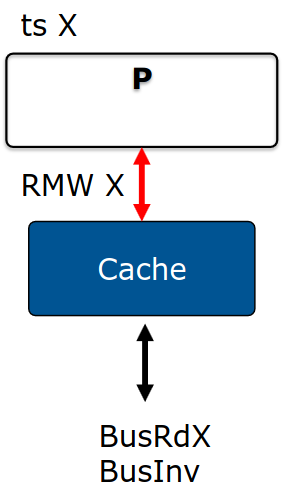
\includegraphics[width=2.5cm]{images/41.png}
        \end{center}
    \end{image}
    \end{tcolorbox}
    We can see now that the problem with TS lock is that the spinning ensure an excessive coherence traffic ! And more processor there is, more traffic increase ! 
    \begin{image}{
         \begin{center}
        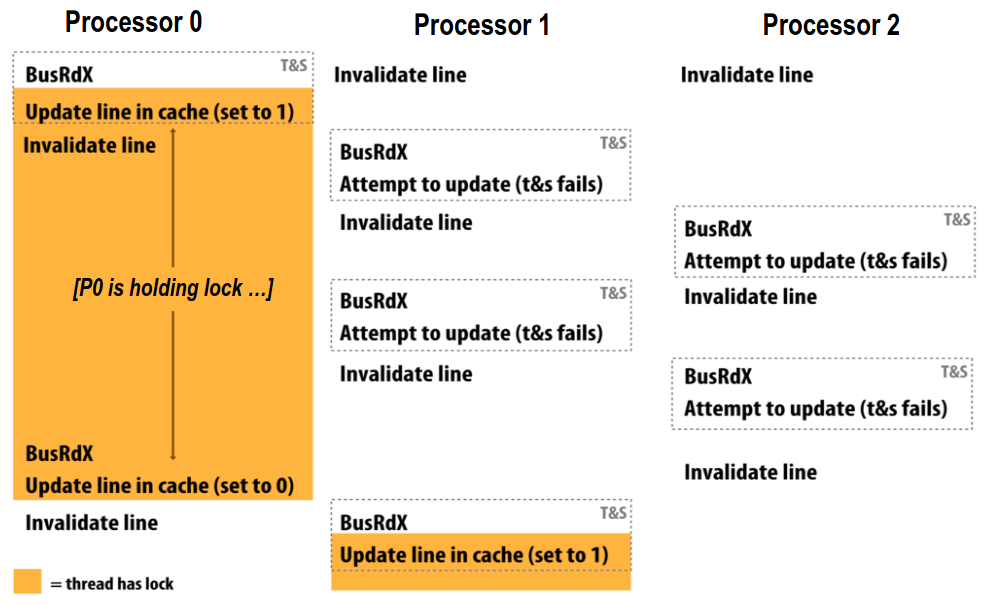
\includegraphics[width=7cm]{images/42.png}
        \end{center}
        }
        \begin{center}
        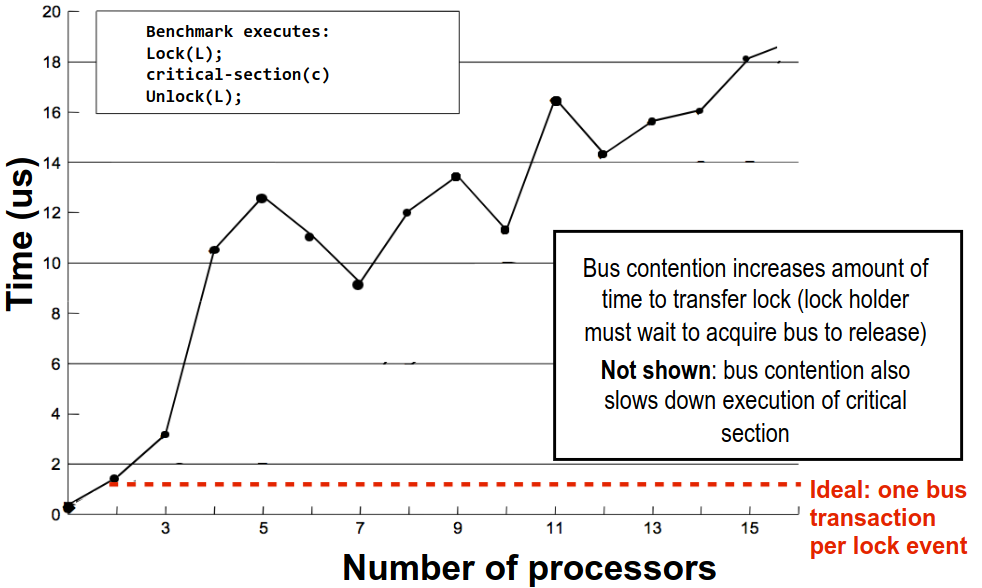
\includegraphics[width=7.5cm]{images/43.png}
        \end{center}
    \end{image}
    \subsubsection{TTS}
    Hopefully there is way to reduce coherence traffic. One way is to test locally.
    \begin{tcolorbox}[rouge]
        The idea behind ``test-and-test-and-set'' (TTS) is to just read classically the lock, if it's 1 (locked), then we just wait. Then, only if it's 0, we read one more time the lock with the TS instruction. So when the processor is waiting, it just does BusRd instead of BusRdX and doesn't invalidate other caches.
        \begin{codeCenter}
        \begin{Ccode}
Test:
    ld r1, mem[addr] // load lock value
    cmp r1, #0
    bnz Test         // compare to 0
Lock:
    ts r1, mem[addr] // load word into R1
    bnz Test         // if 0, lock obtained
Unlock:
    st mem[addr], #0 // store 0 to   
        \end{Ccode}
        \end{codeCenter}
    \end{tcolorbox}

    With TTS we generate much less traffic.
    \begin{center}
    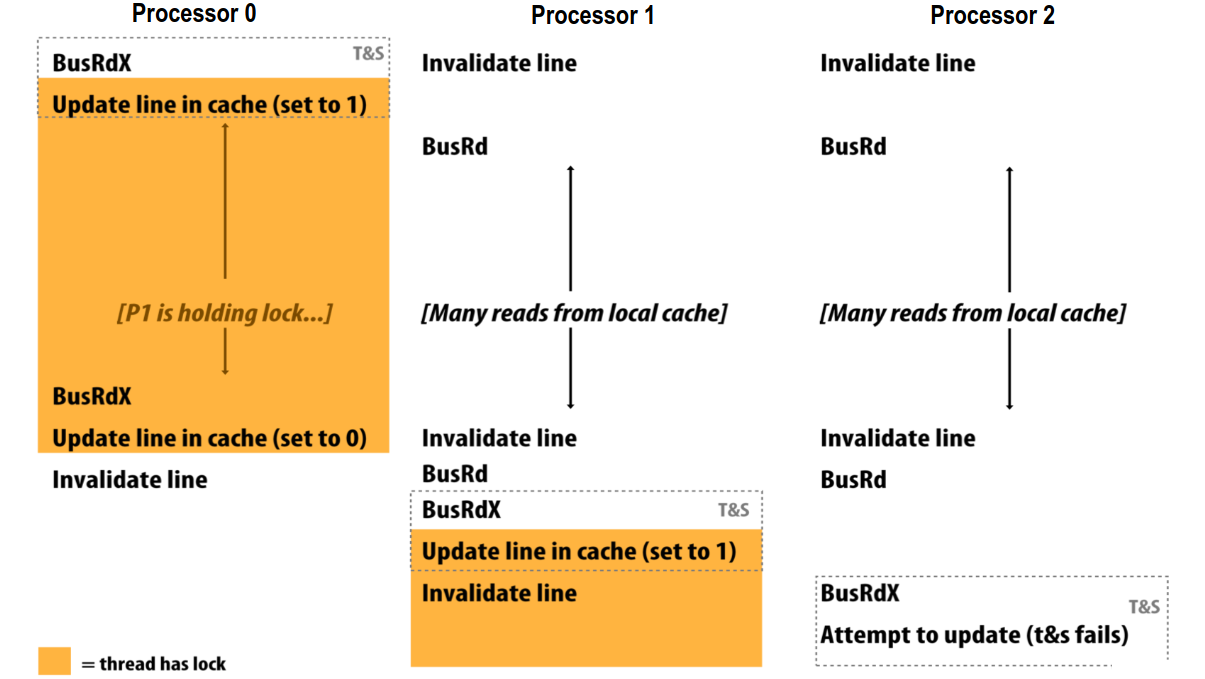
\includegraphics[width=12cm]{images/44.png}
    \end{center}
    TTS have slightly higher latency than TS, but is more scalable and storage cost stay unchanged.
    \subsubsection{TS with exponential back-off}
    \begin{tcolorbox}[rouge]
        Another way to reduce coherence traffic is the TS lock with exponential back-off. The idea is to wait after failing to acquire the lock. To get a balance between lock latency and contention, we increase the time exponentially every fail (1 ms, 2 ms, 4 ms, \ldots). 
    \end{tcolorbox}

    TS with exponential back-off have the same uncontented latency as TS but potentially higher latency under contention. It generates less traffic than TS because it's not continually attempting to acquire lock. It also improve scalability but it can cause sever unfairness: new requester back off for shorter intervals.

    One of the issue with TS and TTS is that they require an instruction that is both a read and a write and this is a challenge for pipelined processors. It must also lock the bus until the RMW completes, so it complicates cache controller logic and two memory accesses per instruction is more difficult to track in CPU pipeline.
    \subsubsection{Load-locked and store-conditional}
    \begin{tcolorbox}[rouge]
        Load-locked (LL) and store-conditional (SC) together provides atomic Read-Modify-Write. The idea is that LL read a value a ``put it under surveillance'', then we can continue to execute some code. After, we can store with SC, that write only if the value hasn't been modified in the memory (by another processor). If it has, we restart from the LL.
    \end{tcolorbox}
    We can use LL/SC to build many types of locks, for example TS:
    \begin{codeCenter}
    \begin{Ccode}
Test_and_Set:
    ldl_l t0, 0(t1)         // load locked, t0 = lock
    bn t0, L1               // if not free, loop
    lda t0, 1(0)            // t0 = 1
    stl_c t0, 0(t1)         // conditional store,
                            // lock = 1
    beq t0, Test_and_Set    // if failed, loop
Release:
    stl 0, 0(t1)
    \end{Ccode}
    \end{codeCenter}
    \begin{tcolorbox}[violet]
    \textbf{Blocking synchronization:}

    The idea of blocking synchronization is that if the progress cannot be make because a resource cannot be acquired, then we free up the core for another thread. We suspend the running thread, the OS schedules another thread to run and the other thread can run and make progress.
    \end{tcolorbox}
    \begin{tcolorbox}[gris]
        \textbf{Busy waiting (spinning) vs blocking synchronization:}
        \begin{itemize}[left=10pt, label=\textbullet]
            \item Busy-waiting is preferable if scheduling overhead is larger than expected wait time, the scheduling overhead is in order of microseconds where it's in nanoseconds for a few spinning operations.
            \item Blocking is preferred if waiting time is significant and there are other tasks that need processor's resources.
        \end{itemize}
    \end{tcolorbox}
        \subsubsection{Coarse/fine-grained locking}
        Coarse grained locks are easy to code, but have bad performance.
        \begin{image}{
            \begin{center}
            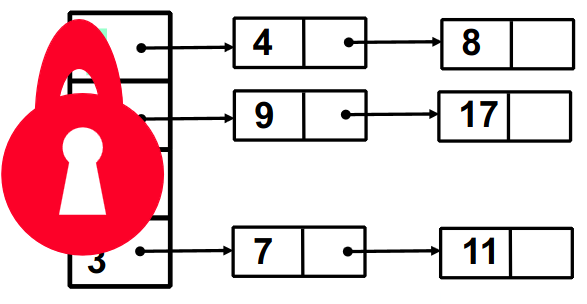
\includegraphics[width=4cm]{images/45.png}
            \end{center}}
        \begin{codeCenter}
        \begin{Ccode}
void editHash(HashTbl tbl, int key) {
    synchronized(tbl) {
    // read objects
    HashObj obj = tbl.get(key);
    // update
    obj.update();
    }
}
        \end{Ccode}
        \end{codeCenter}
        \end{image}
        Fine grained locks are harder to code but have reasonable performance.
        \begin{image}{
            \begin{center}
            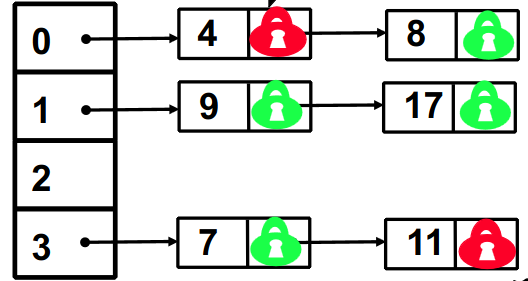
\includegraphics[width=4cm]{images/46.png}
            \end{center}}
        \begin{codeCenter}
        \begin{Ccode}
void editHash(HashTbl tbl, int key) {
    // read objects
    HashObj obj = tbl.get(key);
    synchronized(obj) {
    // update
    obj.update();
    }
}
        \end{Ccode}
        \end{codeCenter}
        \end{image} 
        \begin{center}
        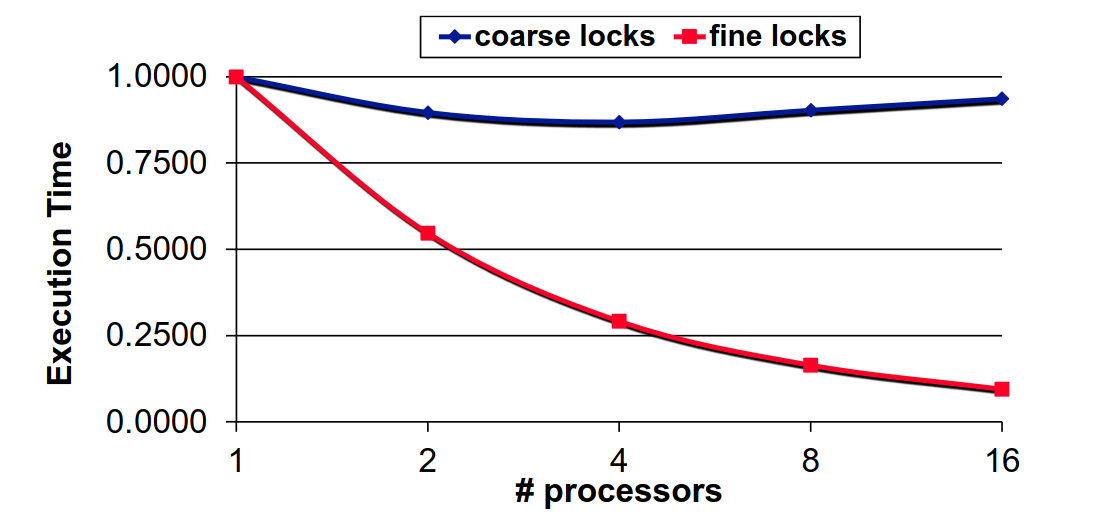
\includegraphics[width=10cm]{images/47.png}
        \end{center}
    \textbf{Localized locking:}
    Localizing locking can sometime not be as easy at it seems, on this example, which pointers do we edit on \lstinline!delete(12)!?
    \begin{center}
    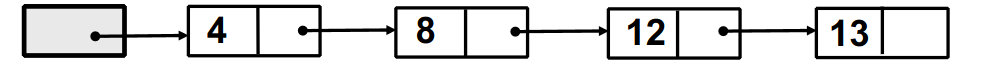
\includegraphics[width=10cm]{images/48.png}
    \end{center}
    The right answer is that we have to lock 8 and 12 because 8\textrightarrow next will now point on 13. To ensure that we get both locks, we grab locks as we traverse the list and we don't release \lstinline!cur! until we have \lstinline!cur->next!. Otherwise, another thread could delete it, making our behavior undefined. This is called hand over hand locking.
    
    \begin{tcolorbox}[violet]
        
    
    Locks have other problems!
    
    \begin{itemize}[left=10pt, label=\textbullet]
        \item \textbf{Priority inversion:} It's when a low-priority process is preempted while holding a lock needed by a high-priority process.
        \item \textbf{Convoying:} It's when a thread is holding a lock and gets swap out by the OS. Then all other threads that are waiting for the lock need to wait.
        \item \textbf{Lock composability:} It's when a thread contains several locks, it can lead to deadlock or livelock if it's implemented incorrectly.
    \end{itemize}
    \end{tcolorbox}
    Here is an example of lock composability which is the major problem in most modern systems. If we have a code that lock successively two objects like this: 

\vspace{0.5em}
\begin{minipage}{0.5\textwidth}
    
    \begin{codeCenter}
    \begin{Ccode}
// P0
objA = tbl.get(1);
objB = tbl.get(2);
synchronized(objA){
    synchronized(objB){
    \end{Ccode}
    \end{codeCenter}
    
\end{minipage}
\begin{minipage}{0.5\textwidth}
\begin{codeCenter}
\begin{Ccode}
// P1
objA = tbl.get(2);
objB = tbl.get(1);
synchronized(objA){
    synchronized(objB){
\end{Ccode}
\end{codeCenter}
\end{minipage}
Then,

\hypertarget{lock}{}
\begin{center}
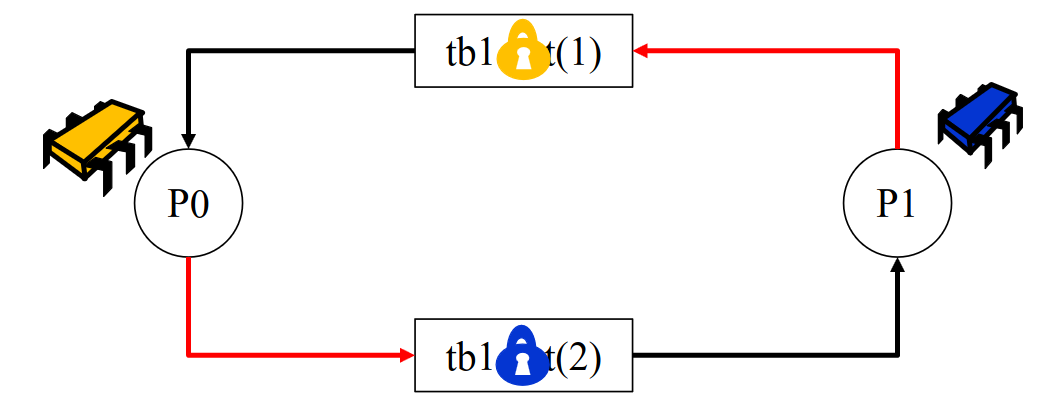
\includegraphics[width=9cm]{images/49.png}
\end{center}
